\documentclass[12pt,a4paper]{article}

% --- Margens conforme modelo ---
\usepackage[lmargin=3cm,rmargin=2cm,tmargin=3cm,bmargin=2cm]{geometry}

% --- Codificação/idioma ---
\usepackage[utf8]{inputenc}
\usepackage[T1]{fontenc}
\usepackage[brazil]{babel}

% --- Fonte Times (equivalente a Times New Roman) ---
\usepackage{newtxtext,newtxmath}

% --- Pacotes úteis ---
\usepackage{enumerate,setspace,graphicx,amsmath,tikz,amsfonts,amssymb}
\usepackage{color}
\usepackage{hyperref}
\usepackage[alf]{abntex2cite}
\usepackage{url}
\usepackage{float}
\usepackage[skip=10pt]{caption}
\usepackage{booktabs}
\usepackage{array}
\usepackage{multirow}
\usepackage{titlesec}

% --- Formatação do artigo ---
\onehalfspacing
\setlength{\parindent}{0pt}   % sem recuo no início do parágrafo
\setlength{\parskip}{6pt}     % 6 pts após cada parágrafo

% --- Legendas ACIMA e com " - " entre rótulo e título ---
\captionsetup{font=small,labelfont=bf}
\captionsetup[figure]{position=above}
\captionsetup[table]{position=above}
\DeclareCaptionLabelSeparator{dash}{\space-\space}
\captionsetup{labelsep=dash}

% --- Numeração das seções: "1." (com ponto) nas seções principais ---
\renewcommand\thesection{\arabic{section}.}
\renewcommand\thesubsection{\arabic{section}.\arabic{subsection}}
\renewcommand\thesubsubsection{\arabic{section}.\arabic{subsection}.\arabic{subsubsection}}

% --- Títulos (12 pt, negrito, alinhados à esquerda, sem espaço extra) ---
\titleformat{\section}{\bfseries\normalsize}{\thesection}{0.5em}{}
\titleformat{\subsection}{\bfseries\normalsize}{\thesubsection}{0.5em}{}
\titleformat{\subsubsection}{\bfseries\normalsize}{\thesubsubsection}{0.5em}{}

% --- Sem espaço extra antes/depois dos títulos ---
\titlespacing*{\section}{0pt}{*0}{*0}
\titlespacing*{\subsection}{0pt}{*0}{*0}
\titlespacing*{\subsubsection}{0pt}{*0}{*0}

% --- Macro para palavras/termos em inglês ---
\newcommand{\eng}[1]{\textit{#1}}

% --- Citação direta longa (NBR 10520): recuo 4 cm, fonte menor, espaço simples, sem aspas ---
\newenvironment{citacao}%
  {\begin{list}{}{\setlength{\leftmargin}{4cm}\setlength{\rightmargin}{0cm}}
   \item \small \singlespacing \noindent}%
  {\end{list}}

\begin{document}
\pagenumbering{gobble} % sem número de páginas

% ============================================================
% Cabeçalho no padrão do modelo (sem capa/folha de rosto)
% ============================================================
{\bfseries Avaliação Comparativa de Algoritmos em Diferentes Linguagens de Programação: Impacto no Desempenho e Eficiência Computacional}

\vspace{6pt}

Guilherme Cavenaghi (Fundação Hermínio Ometto) \texttt{guilherme.cavenaghi@alunos.fho.edu.br}\\
Orientador: Renato Luciano Cagnin (Fundação Hermínio Ometto) \texttt{renato\_cagnin@fho.edu.br}

% ------------------
% Resumo e Palavras-chave
% ------------------
\section*{Resumo}
A eficiência computacional exerce papel central no desenvolvimento de sistemas, sendo influenciada pela escolha da linguagem de programação e pelo paradigma de execução adotado. Este trabalho apresenta uma análise comparativa de algoritmos de diferentes classes de complexidade (P, NP, NP-completo e NP-difícil), implementados em dez linguagens representativas de distintos modelos de tipagem e execução. Foram avaliadas métricas de tempo de execução, uso de memória, consumo de CPU e complexidade de implementação (\eng{SLOC}), em experimentos controlados e repetidos para assegurar confiabilidade estatística. Os resultados indicaram que linguagens compiladas (C, C++ e Rust) tiveram melhor desempenho em tempo e memória, enquanto linguagens interpretadas (Python, JavaScript e TypeScript) destacaram-se pela simplicidade de implementação. A heurística aplicada ao problema NP-completo mostrou-se capaz de obter soluções próximas ao ótimo em frações do tempo demandado pelo algoritmo exato, evidenciando a relevância de técnicas aproximativas. O estudo consolida evidências empíricas que podem apoiar a escolha de tecnologias em diferentes cenários computacionais. Os achados ressaltam o impacto da linguagem e reforçam a importância de pesquisas contínuas, sobretudo em aplicações críticas e ambientes de larga escala, nos quais desempenho, escalabilidade e produtividade influenciam diretamente a qualidade dos sistemas de software.

\vspace{6pt}

\noindent \textbf{Palavras-chave:} algoritmos; linguagens de programação; desempenho computacional; análise de complexidade; eficiência computacional.

% ------------------
% Introdução
% ------------------
\section{Introdução}

O desenvolvimento de software de alta qualidade e desempenho constitui um aspecto central da computação, uma vez que a eficiência afeta diretamente o tempo de execução, o consumo de recursos e a escalabilidade das aplicações. Nesse contexto, a escolha da linguagem de programação emerge como um fator determinante, influenciando a forma como algoritmos são implementados e executados e, consequentemente, o desempenho geral dos sistemas. Embora a lógica algorítmica seja, em essência, independente da linguagem, características como modelo de execução (\eng{interpretado} ou \eng{compilado}), gerenciamento de memória (manual ou automático), tipagem (estática ou dinâmica) e otimizações aplicadas por compiladores ou interpretadores introduzem variações significativas no comportamento prático dos algoritmos \citeonline{sebesta2016}.

Apesar da reconhecida importância do tema, observa-se na literatura uma lacuna quanto a estudos empíricos que abordem comparativamente o impacto das linguagens de programação no desempenho de algoritmos. A maioria dos trabalhos limita-se a análises conceituais ou a relatos de experiências pontuais, carecendo de experimentação controlada e de dados quantitativos robustos que permitam fundamentar decisões de escolha tecnológica em diferentes cenários computacionais. Essa ausência evidencia a necessidade de investigações sistemáticas que transcendam discussões meramente subjetivas e consolidem o conhecimento científico na área.

A relevância desta pesquisa decorre justamente dessa lacuna: orientar desenvolvedores e pesquisadores na seleção de linguagens de programação com base não apenas em critérios subjetivos de preferência ou familiaridade, mas também em evidências empíricas de desempenho, consumo de recursos e complexidade de implementação. Essa fundamentação torna-se especialmente importante em aplicações críticas que demandam alto desempenho e confiabilidade, impactando diretamente a produtividade e a eficiência dos sistemas de software.

A motivação central deste trabalho reside na percepção de que, em um cenário de crescente diversidade de linguagens e de demandas por eficiência, torna-se imperativo compreender como diferentes linguagens se comportam na implementação de algoritmos fundamentais. Essa compreensão possibilita escolhas tecnológicas mais racionais e permite identificar \eng{trade-offs} relevantes entre desempenho e produtividade, contribuindo para o aprimoramento da qualidade de projetos de software em ambientes acadêmicos e industriais.

Diante desse panorama, este trabalho tem como objetivo principal realizar uma análise comparativa do desempenho de algoritmos clássicos pertencentes à classe polinomial, implementados em múltiplas linguagens de programação. Busca-se fornecer uma base empírica que auxilie na tomada de decisões fundamentadas acerca da escolha de linguagem, considerando o impacto de diferentes paradigmas de execução e características de implementação na eficiência computacional. Ademais, a organização deste texto segue orientações de estrutura sugeridas por \citeonline{acconcia2025}, contemplando as seções: introdução, referencial teórico, materiais e métodos, resultados e conclusões.

% ------------------
% Referencial Teórico
% ------------------
\section{Referencial Teórico}

Esta seção apresenta os fundamentos que orientam a análise comparativa realizada. Inicialmente, discute-se a teoria da complexidade computacional, com ênfase nos modelos de computação e nas classes P, NP, NP-completo e NP-difícil. Em seguida, descrevem-se algoritmos representativos utilizados como base empírica. Por fim, apresentam-se critérios de seleção das linguagens e os paradigmas e modelos de execução que influenciam o desempenho de implementações.

\subsection{Teoria da Complexidade Computacional}
A teoria da complexidade computacional tem como objetivo classificar problemas de acordo com os recursos necessários para resolvê-los, como tempo e memória \citeonline{sipser2012}. Essa classificação é essencial para compreender limites práticos e teóricos na execução de algoritmos, servindo de base para a análise comparativa do desempenho em diferentes linguagens de programação. Segundo \citeonline{garey1979}, o estudo da complexidade fornece subsídios para distinguir entre problemas tratáveis e intratáveis, estabelecendo limites matemáticos que orientam escolhas de implementação.

\subsubsection{Modelos de Computação}
O modelo de máquina de Turing constitui a base teórica da complexidade, permitindo a formalização de algoritmos e problemas computacionais. Para um problema de decisão, define-se \(T(n)\) como a função de tempo que representa o número de passos executados para resolver uma entrada de tamanho \(n\). Esse modelo, embora abstrato, é amplamente utilizado para definir limites fundamentais sobre o que pode ou não ser computado \cite{sipser2012}. Outros modelos, como as máquinas RAM (\eng{Random Access Machine}), oferecem maior proximidade com arquiteturas reais, mas mantêm a mesma equivalência de poder computacional \cite{knuth1998}.

O modelo de Turing é também essencial para a definição das classes de complexidade polinomial. A classe P corresponde ao conjunto de problemas que podem ser resolvidos em tempo polinomial por uma máquina de Turing determinística, enquanto a classe NP compreende problemas cujas soluções podem ser verificadas em tempo polinomial nesse mesmo modelo \cite{garey1979, sipser2012}. Assim, as noções de tratabilidade e intratabilidade em ciência da computação derivam diretamente dessa formalização, o que justifica sua presença neste estudo, voltado à comparação empírica do desempenho de algoritmos fundamentais em diferentes linguagens de programação.

\subsubsection{Classes de Complexidade Polinomial}
O presente estudo foca em classes de complexidade polinomial, pois elas fornecem o arcabouço necessário para compreender os resultados obtidos. A Figura~\ref{fig:complexidade} ilustra as principais relações entre essas classes:

\begin{itemize}
  \item \textbf{Classe P}: Problemas solucionáveis por algoritmos determinísticos em tempo polinomial. Representam problemas tratáveis na prática, como o \eng{MergeSort} (\(O(n \log n)\)), que é amplamente descrito em literatura clássica de algoritmos \citeonline{knuth1998}.
  \item \textbf{Classe NP}: Problemas cujas soluções podem ser verificadas em tempo polinomial, ainda que não haja algoritmo determinístico conhecido para resolvê-los em tempo polinomial. Exemplo clássico: fatoração de inteiros, relevante em criptografia moderna \citeonline{rivest1978}.
  \item \textbf{Classe NP-completo}: Problemas para os quais qualquer outro problema em NP pode ser reduzido em tempo polinomial. Exemplo: Problema da Mochila (\eng{Knapsack}), que é referência em problemas de otimização combinatória \citeonline{garey1979}.
  \item \textbf{Classe NP-difícil}: Problemas no mínimo tão difíceis quanto qualquer problema de NP, podendo ou não ser verificáveis em tempo polinomial. Incluem problemas indecidíveis, como o da Parada (\eng{Halting Problem}), para o qual não existe algoritmo geral \citeonline{sipser2012}.
\end{itemize}

\begin{figure}[H]
  \caption{Diagrama das classes de complexidade P, NP, NP-completo e NP-difícil.}
  \centering
  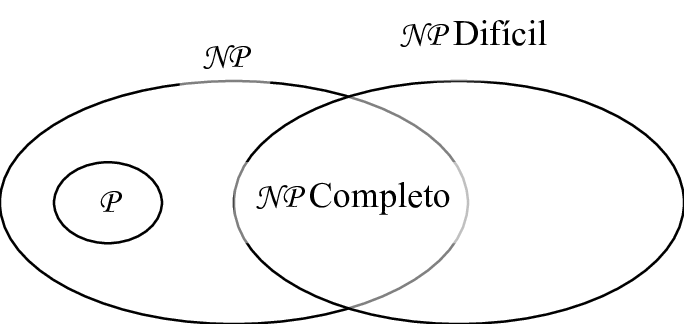
\includegraphics[width=0.5\textwidth]{img/relacaoDeConjuntos.png}
  \label{fig:complexidade}
  \\ \small Fonte: Adaptado de \citeonline{article}.
\end{figure}

\subsection{Algoritmos Fundamentais}
Para avaliar o impacto das linguagens no desempenho, foram selecionados algoritmos representativos das diferentes classes polinomiais, considerando tanto sua relevância teórica quanto aplicabilidade prática. Conforme \citeonline{pressman2016}, a escolha adequada de algoritmos influencia diretamente tempo de execução, consumo de recursos e escalabilidade das aplicações. A seleção também foi guiada pela teoria da complexidade, de modo que cada classe polinomial esteja associada a um exemplo canônico, amplamente discutido na literatura.

\subsubsection{Ordenação}
O algoritmo \eng{MergeSort} é representativo da classe P, com complexidade \(O(n \log n)\). Problemas dessa classe podem ser resolvidos em tempo polinomial por uma máquina de Turing determinística \cite{sipser2012}. A escolha do MergeSort se deve ao fato de ser um dos algoritmos de ordenação mais estudados, com análise matemática bem estabelecida \cite{knuth1998}. Além disso, sua popularidade e ampla utilização em sistemas reais tornam-no adequado como \eng{benchmark} para linguagens compiladas e interpretadas, permitindo observar diferenças de desempenho em cenários considerados tratáveis \cite{tanenbaum2015}.

\subsubsection{Problemas de Otimização e Fatoração}
O Problema da Mochila (\eng{Knapsack}) foi escolhido por representar a classe NP-completo. Problemas desse tipo podem ser verificados em tempo polinomial por uma máquina de Turing determinística, mas não se conhece algoritmo eficiente de resolução geral \cite{garey1979}. O Knapsack é um caso clássico de busca combinatória, utilizado em contextos de otimização e tomada de decisão, o que o torna relevante para avaliar o impacto das linguagens em cenários de explosão combinatória.

Já a fatoração de inteiros (\eng{Factoring}), pertencente à classe NP, é amplamente estudada devido à sua importância em criptografia, especialmente na segurança de sistemas como o RSA \cite{rivest1978}. A escolha desse problema permite explorar como diferentes linguagens lidam com operações matemáticas de alta complexidade prática, mas que permanecem verificáveis em tempo polinomial. Isso fornece um contraponto ao Knapsack, situando o estudo em diferentes níveis da classe NP.

\subsubsection{Problemas Indecidíveis}
O Problema da Parada (\eng{Halting Problem}), embora indecidível em sua formulação geral, representa a classe NP-difícil em sua vertente teórica. Nesse tipo de problema, não existe algoritmo capaz de resolvê-lo em todos os casos possíveis \cite{sipser2012}. No entanto, é possível considerar instâncias restritas e simuláveis, de forma a observar o comportamento das linguagens em termos de tempo de execução e uso de memória. Sua inclusão reforça a relação entre limites teóricos da computabilidade e observações empíricas, permitindo avaliar até que ponto a escolha da linguagem pode mitigar ou evidenciar a complexidade intrínseca dos problemas.

\subsection{Linguagens de Programação}
A linguagem de programação exerce impacto significativo na implementação de algoritmos, afetando diretamente tempo de execução, uso de memória e esforço de desenvolvimento. Estudos empíricos demonstram que linguagens distintas podem produzir resultados divergentes em termos de eficiência computacional, mesmo implementando o mesmo algoritmo \cite{prechelt2000, nanz2015, ray2017}. Essa diversidade justifica a análise comparativa proposta neste trabalho, pois permite observar como características de cada linguagem interagem com diferentes classes de complexidade.

\subsubsection{Paradigmas e Modelos de Execução}
Os paradigmas de programação influenciam a forma como problemas são estruturados e resolvidos, afetando diretamente o tempo de execução, o consumo de recursos e a legibilidade do código \citeonline{sebesta2016}. Entre os aspectos mais relevantes destacam-se:

\begin{itemize}
  \item \textbf{Modelo de execução}: compilado ou interpretado. Em problemas da classe P, como o \eng{MergeSort}, linguagens compiladas tendem a explorar otimizações de baixo nível, reduzindo o tempo de execução. Já em problemas da classe NP-completo, como o \eng{Knapsack}, a vantagem de compilação pode se diluir frente à explosão combinatória, mas ainda impacta significativamente a escalabilidade das instâncias \cite{aho2007}.
  \item \textbf{Tipagem}: estática ou dinâmica. Tipagens estáticas, comuns em linguagens compiladas, podem evitar erros e otimizar verificações em tempo de compilação \cite{sebesta2016}. Por outro lado, tipagens dinâmicas, típicas de linguagens interpretadas como Python e JavaScript, oferecem maior flexibilidade, mas podem gerar sobrecarga em execuções repetitivas de algoritmos NP ou NP-completos, impactando desempenho em comparação a linguagens com checagem antecipada de tipos \cite{tanenbaum2015}.
  \item \textbf{Gerenciamento de memória}: manual ou automático. Em algoritmos intensivos em memória, como aqueles que implementam o \eng{Knapsack} ou simulam instâncias do \eng{Halting Problem}, o controle manual (C, C++) pode reduzir sobrecarga, mas aumenta a complexidade do código. Já o gerenciamento automático (Java, C\#, Go) facilita a implementação, porém pode introduzir pausas de coleta de lixo (\eng{garbage collection}), afetando medições de desempenho \cite{tanenbaum2015}.
\end{itemize}

Dessa forma, os paradigmas e modelos de execução não apenas influenciam a forma como os algoritmos são implementados, mas também determinam o comportamento observado em termos de desempenho, consumo de recursos e escalabilidade. Estudos comparativos demonstram que linguagens distintas podem apresentar diferenças substanciais de performance mesmo ao executar algoritmos idênticos, reforçando a necessidade de análises empíricas \cite{prechelt2000}. Em particular, \citeonline{nanz2015} evidenciam que, mesmo em tarefas simples e equivalentes, a escolha da linguagem pode resultar em variações significativas no tempo de execução e no consumo de memória. De forma complementar, \citeonline{ray2017} mostram que tais diferenças não se limitam a cenários controlados, mas também impactam a qualidade do software em larga escala, afetando manutenibilidade e propensão a erros.

Assim, compreender a interação entre paradigmas, modelos de execução e classes de complexidade é essencial para fundamentar escolhas tecnológicas. A análise empírica proposta neste trabalho busca justamente oferecer evidências que complementem a teoria, mostrando como características das linguagens influenciam a execução de algoritmos em cenários reais.

% ------------------
% Materiais e Métodos
% ------------------
\section{Materiais e Métodos}

Esta seção descreve o ambiente de experimentação e os procedimentos utilizados na condução dos testes comparativos. São apresentados os recursos de hardware e software empregados, as métricas consideradas na análise, os conjuntos de dados adotados e as etapas que compuseram o processo experimental, de forma a garantir a reprodutibilidade do estudo.

\subsection{Critérios de Seleção}
As linguagens foram escolhidas com base em três critérios principais:
\begin{itemize}
  \item \textbf{Popularidade}: índices amplamente reconhecidos como o \eng{TIOBE Index}, o \eng{GitHub Octoverse} e a \eng{Stack Overflow Developer Survey}.
  \item \textbf{Diversidade de paradigmas}: linguagens compiladas (C, C++, Rust), interpretadas (Python, JavaScript) e híbridas (Java, C\#, Go, Kotlin, TypeScript), conforme \eng{Sebesta} \citeonline{sebesta2016}.
  \item \textbf{Aplicabilidade acadêmica e industrial}: presença em cursos universitários, bibliotecas científicas e projetos de larga escala \cite{pressman2016}.
\end{itemize}

\subsection{Ambiente Experimental}
Os experimentos foram realizados em máquina dedicada com as seguintes especificações:
\begin{itemize}
  \item \textbf{Processador}: Intel Core i7-1165G7 (11ª geração), 2.80 GHz.
  \item \textbf{Memória RAM}: 16 GB DDR4 (2667 MHz).
  \item \textbf{Vídeo}: Intel Iris Xe Graphics.
  \item \textbf{Sistema Operacional}: \eng{Ubuntu 24.04 LTS}.
\end{itemize}

Para reduzir interferências externas, os testes foram executados em modo de alto desempenho, sem aplicações concorrentes além dos serviços essenciais do sistema e cada execução foi realizada em console dedicado, garantindo uniformidade no ambiente experimental.

\subsection{Métricas}
Foram avaliados três aspectos principais:
\begin{itemize}
  \item \textbf{Tempo de execução (\eng{Wall Clock})}: média de 30 execuções consecutivas, medidas com \texttt{/usr/bin/time}.
  \item \textbf{Uso de memória (RSS)}: pico de memória residente, obtido também via \texttt{/usr/bin/time}.
  \item \textbf{Complexidade de implementação}: número de linhas de código fonte (\eng{SLOC}), medido com a ferramenta \texttt{cloc}, e complexidade ciclomática, calculada com a ferramenta \texttt{lizard}.
\end{itemize}

\subsection{Conjuntos de Dados}
Todos os conjuntos de dados utilizados nos experimentos foram gerados sinteticamente por scripts especializados desenvolvidos para cada problema, de modo a garantir instâncias compatíveis com a formulação de cada algoritmo e plena reprodutibilidade. Os geradores utilizam geradores pseudoaleatórios com \emph{seed} fixa registrada nos respectivos scripts; as seeds e parâmetros de geração encontram-se documentados no repositório complementar (diretório \texttt{datasets/}).

Para fins de reprodutibilidade, cada gerador aceita argumentos de entrada típicos como \texttt{--seed}, \texttt{--n} (tamanho) e \texttt{--out} (arquivo de saída). A seguir descreve-se a estratégia aplicada para cada classe de problema e um exemplo de comando de geração.

\begin{itemize}
  \item \textbf{Classe P -- \eng{MergeSort}}: o gerador produz vetores de inteiros em três padrões:
    (i) totalmente ordenados, (ii) parcialmente ordenados (50\% dos elementos embaralhados) e (iii) totalmente aleatórios. Os valores inteiros são sorteados em uma faixa proporcional a \(n\) (por exemplo, \([0, 10 \cdot n]\)) e a ordem/fragmentação é controlada por parâmetros.

  \item \textbf{Classe NP -- Fatoração de inteiros (\eng{Factoring})}: o gerador cria inteiros compostos como produto de dois primos pseudoaleatórios. Para cada \(n\) a função controla o tamanho (número de bits ou dígitos) dos fatores primos para produzir números de ordem de grandeza adequada. A seed garante a reprodutibilidade das escolhas de primos.

  \item \textbf{Classe NP-completo -- Mochila (\eng{Knapsack})}: o gerador produz instâncias com um conjunto de itens, cada um contendo peso e valor inteiros, além de uma capacidade da mochila. Os parâmetros incluem a razão entre capacidade e soma de pesos (densidade), faixa de pesos/valores e distribuição (uniforme, exponencial, etc.). Foram geradas variações de baixa e alta densidade para cada.

  \item \textbf{Classe NP-difícil -- Problema da Parada (\eng{Halting})}: como o problema é indecidível em geral, o gerador produz programas simples em pseudocódigo com três categorias: (i) parada imediata, (ii) parada observável em tempo limitado (com laços limitados), e (iii) instâncias construídas para evidenciar comportamento potencialmente não-terminante (por exemplo, laços dependentes de condição não determinística). Essas instâncias são usadas apenas para avaliar comportamento empírico e limites práticos.
\end{itemize}

Os arquivos de saída foram gravados em formato \texttt{JSON} com esquema uniforme (identificador da instância, parâmetros de geração e dados necessários para a execução do algoritmo). As seeds utilizadas em cada execução e os parâmetros concretos (por exemplo, faixas numéricas, densidades e taxas) estão registrados em um arquivo \texttt{datasets/README.md} incluído no repositório, garantindo que qualquer pesquisador possa regenerar as mesmas instâncias.

Os tamanhos adotados para os experimentos foram:
\begin{itemize}
  \item \textbf{Pequeno}: \(n = 10^3\).
  \item \textbf{Médio}: \(n = 10^4\).
  \item \textbf{Grande}: \(n = 10^5\).
\end{itemize}

Observação: para problemas cuja execução exata é inviável em níveis maiores (por exemplo, solução exata do \eng{Knapsack} em \eng{large}), aplicou-se uma política experimental (descrita adiante) que evita execuções proibitivamente longas.

\subsection{Procedimentos Experimentais}
O processo experimental foi organizado em três etapas principais: (i) geração de instâncias, (ii) compilação/execução e monitoramento, e (iii) armazenamento e análise dos resultados. Abaixo estão os procedimentos detalhados, refletindo os scripts e knobs utilizados.

\begin{enumerate}
  \item \textbf{Geração de datasets}: antes de qualquer execução, as instâncias foram geradas pelos scripts descritos na subseção anterior. Para cada combinação \eng{problema} $\times$ \eng{tamanho} foi executado o gerador com uma \emph{seed} fixa e parâmetros documentados; os arquivos resultantes foram versionados no repositório para rastreabilidade.

  \item \textbf{Implementação e preparação}: os algoritmos foram implementados em todas as linguagens avaliadas usando apenas bibliotecas padrão. Os nomes dos arquivos fonte e o mapeamento linguagem$\to$arquivo seguem a organização do repositório (diretório \texttt{algorithms/\{linguagem\}/}). Antes da execução, o sistema verifica presença de compiladores/runtimes necessários e compila quando aplicável (flags padrão usadas: \texttt{gcc -O2}, \texttt{g++ -O2}, \texttt{rustc -C opt-level=3}, compilação Java/Kotlin padrão, etc.).

  \item \textbf{Execução e monitoramento}: cada execução foi conduzida pelo script de coleta de métricas (\texttt{coleta\_metricas.py}), que:
    \begin{itemize}
      \item executa o binário/interpretador com a instância gerada;
      \item monitora consumo de CPU e memória residente (RSS) por amostragem via \texttt{psutil} (parâmetros ajustáveis via variáveis de ambiente como \texttt{SAMPLE\_INTERVAL} e \texttt{TIMEOUT\_SEC});
      \item agrega tempos de CPU em usuário/sistema (a partir de \texttt{psutil} e \texttt{resource}) e mede \eng{wall time} (tempo de parede);
      \item captura \texttt{stdout}/\texttt{stderr}, \texttt{exit\_code} e campos específicos do problema (por exemplo, \texttt{valor\_objetivo} para \eng{knapsack});
      \item aplica política de skip para execuções exatas de \eng{np-completo} no bucket \eng{large} para evitar tempos impraticáveis.
    \end{itemize}

  \item \textbf{Repetições e controle de variabilidade}: para cada combinação \eng{linguagem} $\times$ \eng{problema} $\times$ \eng{tamanho} foram realizadas 30 repetições independentes (excetuando casos pulados por política). Antes e após cada execução o script registra níveis de ociosidade do sistema (\eng{idle CPU} e uso de memória) para avaliar interferências externas.

  \item \textbf{Registro e formato de saída}: os resultados de cada execução são adicionados a um arquivo \texttt{JSON} acumulativo (\texttt{resultados/metricas.json}) contendo metadados do sistema (distribuição, kernel, arquitetura, número de cores, memória total), parâmetros da execução, medidas agregadas (média e pico) e séries quando aplicável.

  \item \textbf{Análise estatística}: a partir do conjunto de execuções foram calculadas medidas descritivas (média e desvio-padrão) por combinação de fatores, permitindo comparar desempenho entre linguagens, problemas e tamanhos de entrada. Valores relativos a variáveis de ambiente e seeds utilizadas estão disponibilizados no repositório para reprodução integral.
\end{enumerate}

\subsection{Procedimentos Experimentais}
O processo experimental foi conduzido de forma padronizada para todas as linguagens e algoritmos, conforme as seguintes etapas:

\begin{enumerate}
  \item \textbf{Implementação}: cada problema foi implementado em todas as linguagens avaliadas, utilizando apenas bibliotecas padrão ou recursos nativos, de modo a evitar influências externas no desempenho.

  \item \textbf{Compilação e execução}: os programas foram compilados ou interpretados com ferramentas oficiais disponíveis no \eng{Ubuntu 24.04 LTS}, adotando parâmetros padrão de cada linguagem (por exemplo, \texttt{gcc -O2}, \texttt{javac}, \texttt{python3}, \texttt{node}, etc.).

  \item \textbf{Repetições}: para cada combinação \eng{linguagem $\times$ problema $\times$ tamanho de entrada}, foram realizadas 30 execuções independentes, a fim de reduzir o impacto de flutuações ocasionais do sistema.

  \item \textbf{Coleta de métricas}: em cada execução foram registrados automaticamente o tempo de execução (\eng{Wall Clock}) e o pico de uso de memória residente (RSS), utilizando a ferramenta \texttt{/usr/bin/time}. As métricas de implementação (\eng{SLOC} e complexidade ciclomática) foram extraídas estaticamente pelas ferramentas \texttt{cloc} e \texttt{lizard}.

  \item \textbf{Registro dos resultados}: os dados coletados foram armazenados em formato \eng{JSON}, incluindo metadados sobre a linguagem, problema, tamanho de entrada, repetição e métricas obtidas.

  \item \textbf{Análise estatística}: a partir dos resultados brutos, foram calculadas medidas descritivas (média e desvio-padrão), permitindo comparação entre linguagens, problemas e tamanhos de entrada.
\end{enumerate}

% ------------------
% Resultados
% ------------------
\section{Resultados}

Nesta seção são apresentados e analisados os resultados obtidos a partir da execução sistemática dos algoritmos implementados. Os experimentos foram conduzidos com diferentes linguagens de programação e classes de complexidade (P, NP, NP-completo e NP-difícil), considerando quatro dimensões principais de avaliação: tempo de execução, utilização de CPU, consumo de memória e qualidade da solução heurística. Adicionalmente, é apresentada uma análise quantitativa em relação ao número de linhas de código fonte (\eng{SLOC - Source Lines of Code}), com o objetivo de avaliar a expressividade sintática e o esforço de implementação requerido por cada linguagem.

\subsection{Tempo de Execução}

O tempo de execução médio, acompanhado do respectivo Desvio Padrão, dos algoritmos foi avaliado em três categorias de tamanho de \eng{dataset} (\eng{small}, \eng{medium}, \eng{large}). Os resultados agregados englobam algoritmos de diferentes classes de complexidade, com exceção dos problemas NP-completos, que foram analisados em separado devido às suas exigências computacionais exponenciais.

\begin{figure}[H]
\caption{Tempo médio de execução versus tamanho do \eng{dataset}.}
\centering
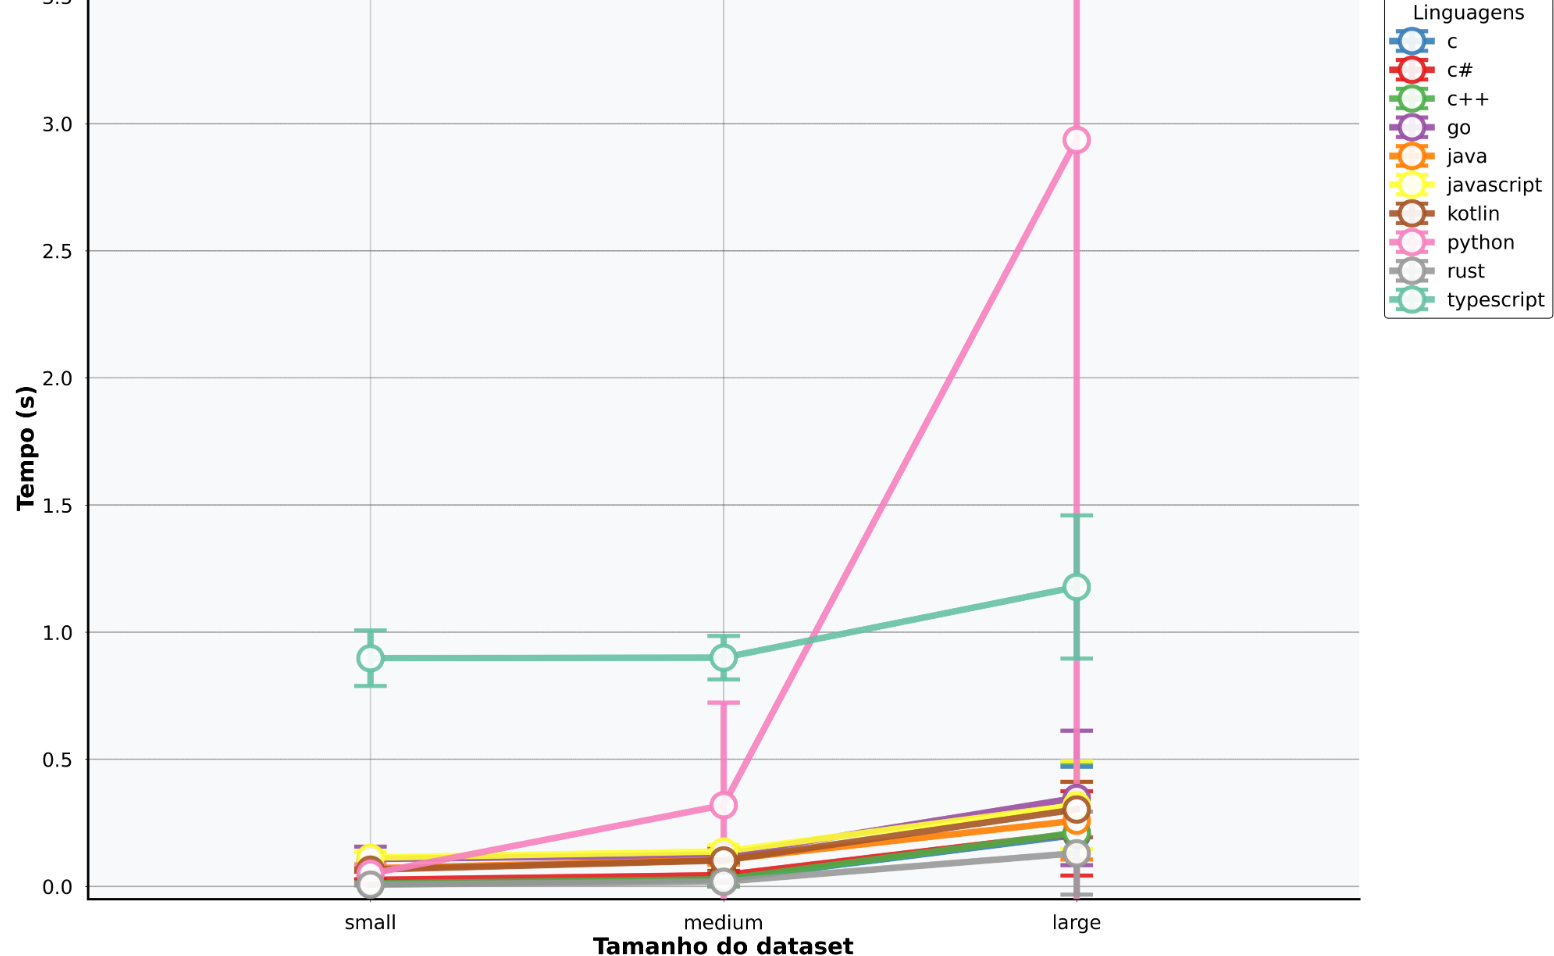
\includegraphics[width=\textwidth]{img/tempo_vs_tamanho.png}
\label{fig:tempo_execucao}
\centering
\small Fonte: Autor.
\end{figure}

\begin{table}[H]
  \caption{Tempo médio de execução (s) e desvio-padrão por linguagem e tamanho do \eng{dataset}.(M: Média, DP: Desvio-Padrão)}
  \centering
  \resizebox{\textwidth}{!}{%
  \begin{tabular}{l|cc|cc|cc|cc|cc|cc|cc|cc|cc|cc|cc|cc}
    \toprule
    \textbf{Tamanho} & \multicolumn{2}{c|}{\textbf{C}} & \multicolumn{2}{c|}{\textbf{C\#}} & \multicolumn{2}{c|}{\textbf{C++}} & \multicolumn{2}{c|}{\textbf{Go}} & \multicolumn{2}{c|}{\textbf{Java}} & \multicolumn{2}{c|}{\textbf{JS}} & \multicolumn{2}{c|}{\textbf{Kotlin}} & \multicolumn{2}{c|}{\textbf{Python}} & \multicolumn{2}{c|}{\textbf{Rust}} & \multicolumn{2}{c}{\textbf{TS}} \\
    \midrule
    & M & DP  & M & DP & M & DP & M & DP & M & DP & M & DP & M & DP & M & DP & M & DP & M & DP \\
    \midrule
    \eng{small}  & 0.01 & 0.00 & 0.03 & 0.00 & 0.01 & 0.01 & 0.11 & 0.05 & 0.07 & 0.01 & 0.11 & 0.02 & 0.07 & 0.01 & 0.05 & 0.04 & 0.01 & 0.00 & 0.90 & 0.11 \\
    \eng{medium} & 0.03 & 0.03 & 0.04 & 0.02 & 0.03 & 0.03 & 0.12 & 0.03 & 0.10 & 0.02 & 0.14 & 0.03 & 0.10 & 0.01 & 0.32 & 0.40 & 0.02 & 0.02 & 0.90 & 0.09 \\
    \eng{large}  & 0.20 & 0.27 & 0.21 & 0.17 & 0.21 & 0.28 & 0.35 & 0.26 & 0.26 & 0.26 & 0.32 & 0.17 & 0.30 & 0.11 & 2.94 & 3.95 & 0.13 & 0.16 & 1.18 & 0.28 \\
    \bottomrule
  \end{tabular}%
  }
\label{fig:tempo_execucao}
\centering
\small Fonte: Autor.
\end{table}

Os resultados demonstram uma correlação significativa entre o paradigma de execução das linguagens e seu desempenho temporal. Linguagens compiladas diretamente para código nativo (C, C++ e Rust) apresentaram os menores tempos de execução, com médias variando entre 0.01 segundos (instâncias pequenas) e 0.21 segundos (instâncias grandes), evidenciando superioridade em eficiência computacional. Rust merece destaque particular por combinar alta performance com garantias de segurança de memória, alcançando tempos comparáveis a C/C++ com valores de Desvio Padrão inferiores, indicando comportamento de execução mais consistente e previsível.
Linguagens que operam em máquinas virtuais gerenciadas (Java, Kotlin, C#) demonstraram desempenho intermediário, com tempos de execução 2 a 7 vezes superiores às linguagens nativas em instâncias pequenas, porém mantendo boa escalabilidade para problemas de maior complexidade. Java e Kotlin apresentaram valores de Desvio Padrão relativamente baixos (0.01-0.26), sugerindo comportamento temporal estável sob diferentes condições de carga computacional.
Python exibiu a maior variabilidade temporal (Desvio Padrão até 3.95) e crescimento exponencial em instâncias grandes (2.94 segundos na média), refletindo limitações inerentes a linguagens interpretadas para execução de algoritmos computacionalmente complexos. JavaScript e TypeScript apresentaram comportamento divergente: enquanto JavaScript demonstrou desempenho temporal razoável, TypeScript foi consistentemente mais lento (até 1.18 segundos), possivelmente devido aos overheads adicionais do processo de transpilação e verificação de tipos em tempo de execução.

\subsection{Uso de CPU}
A Figura~\ref{fig:cpu} ilustra o consumo máximo de CPU normalizado pelo tamanho da instância processada. Linguagens com ambientes de execução mais complexos (Java, Kotlin) apresentam utilização intensiva de CPU em instâncias médias e grandes, em contraste direto com C e C++, que demonstram comportamento de utilização mais estável e eficiente. O Desvio Padrão calculado evidencia que linguagens interpretadas possuem maior variabilidade na utilização de recursos, indicando ocorrência de picos de processamento durante fases específicas da execução.

\begin{figure}[H]
  \caption{Consumo máximo de CPU normalizada por tamanho.}
  \centering
  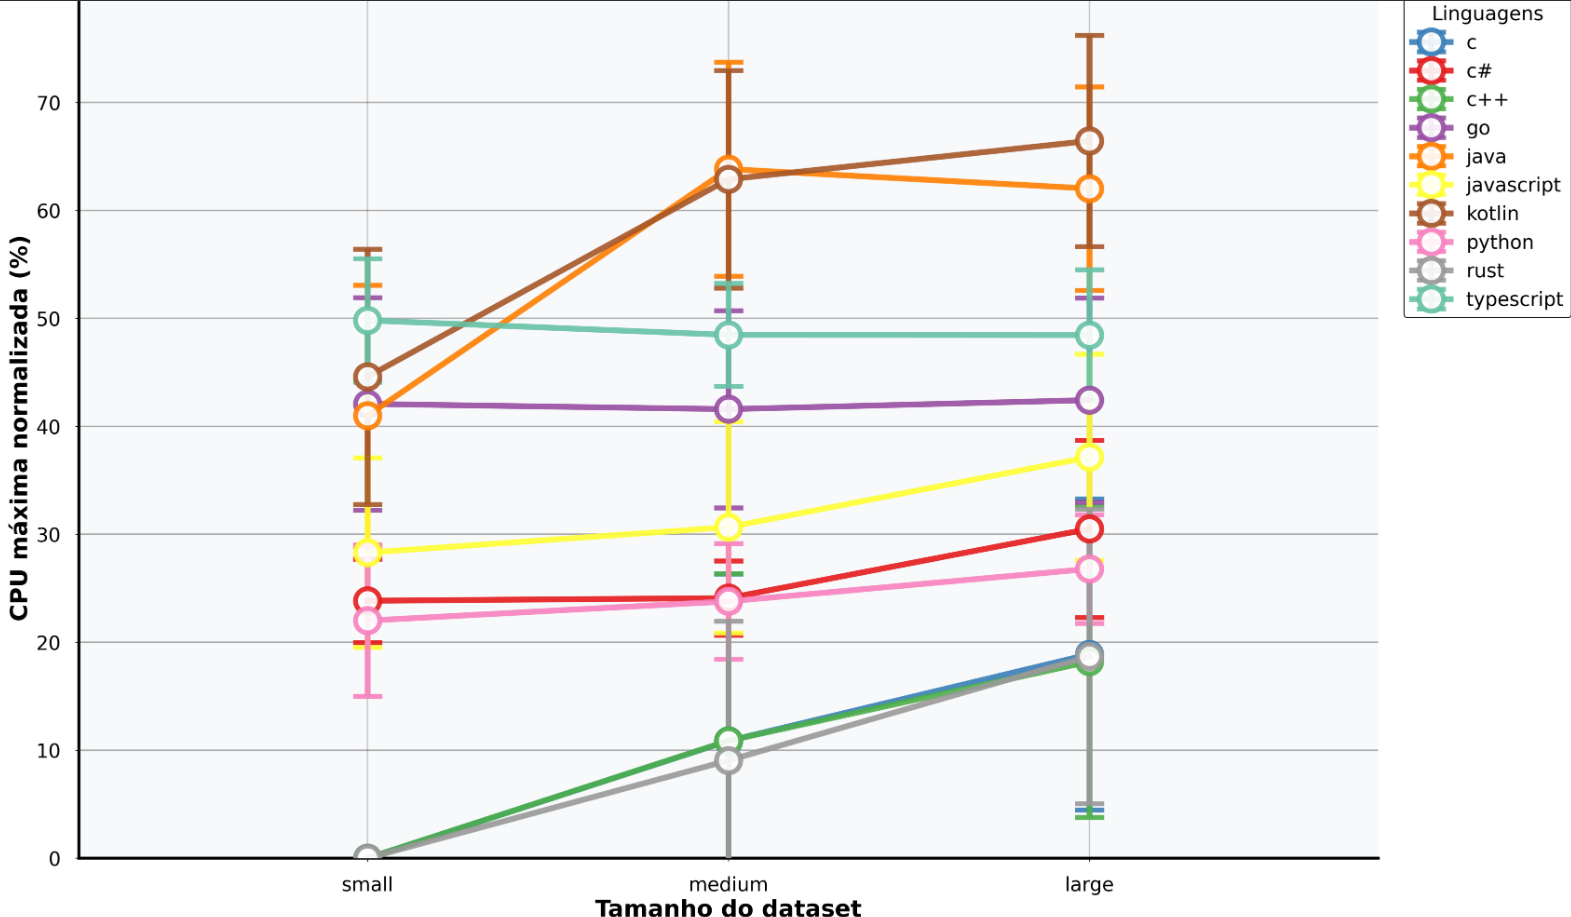
\includegraphics[width=\textwidth]{img/cpu_vs_tamanho.png}
  \label{fig:cpu}
  \small Fonte: Autor.
\end{figure}

\begin{table}[H]
  \caption{Consumo máximo de CPU normalizada (\%) por linguagem e tamanho de \eng{dataset}.(M: Média, DP: Desvio-Padrão)}
  \centering
  \resizebox{\textwidth}{!}{%
  \begin{tabular}{l|cc|cc|cc|cc|cc|cc|cc|cc|cc|cc|cc|cc}
    \toprule
    \textbf{Tamanho} & \multicolumn{2}{c|}{\textbf{C}} & \multicolumn{2}{c|}{\textbf{C\#}} & \multicolumn{2}{c|}{\textbf{C++}} & \multicolumn{2}{c|}{\textbf{Go}} & \multicolumn{2}{c|}{\textbf{Java}} & \multicolumn{2}{c|}{\textbf{JS}} & \multicolumn{2}{c|}{\textbf{Kotlin}} & \multicolumn{2}{c|}{\textbf{Py}} & \multicolumn{2}{c|}{\textbf{Rust}} & \multicolumn{2}{c}{\textbf{TS}} \\
    \midrule
    & M & DP & M & DP & M & DP & M & DP & M & DP & M & DP & M & DP & M & DP & M & DP & M & DP \\
    \midrule
    \eng{small}  & 0.00 & 0.00 & 23.84 & 3.86 & 0.00 & 0.00 & 42.08 & 9.85 & 40.99 & 12.08 & 28.30 & 8.78 & 44.59 & 11.82 & 22.00 & 7.01 & 0.00 & 0.00 & 49.82 & 5.72 \\
    \eng{medium} & 10.86 & 15.46 & 24.09 & 3.43 & 10.88 & 15.48 & 41.59 & 9.14 & 63.83 & 9.91 & 30.66 & 9.79 & 62.89 & 10.08 & 23.79 & 5.35 & 9.05 & 12.91 & 48.47 & 4.76 \\
    \eng{large}  & 18.88 & 14.40 & 30.50 & 8.21 & 18.21 & 14.42 & 42.43 & 9.46 & 62.03 & 9.42 & 37.15 & 9.55 & 66.44 & 9.78 & 26.79 & 5.04 & 18.70 & 13.65 & 48.45 & 6.07 \\
    \bottomrule
  \end{tabular}%
  }
\label{fig:tempo_execucao}
\centering
\small Fonte: Autor.
\end{table}

A análise do consumo de recursos de processamento revela padrões arquiteturais importantes sobre a eficiência computacional. Linguagens nativas (C, C++, Rust) demonstraram controle excepcional sobre recursos de CPU, com utilização próxima de 0\% em instâncias pequenas e crescimento moderado em instâncias maiores (18\%--19\%). Seus elevados valores de Desvio Padrão (12--15) indicam que, embora extremamente eficientes, essas linguagens podem apresentar picos pontuais de utilização de CPU quando necessário, aproveitando integralmente os recursos computacionais disponíveis mediante demanda.

Linguagens que utilizam coleta automática de lixo (Java, Kotlin, Go) apresentaram padrão diametralmente oposto: alto consumo mesmo em tarefas computacionalmente simples (40\%--66\%), com relativa estabilidade operacional (Desvio Padrão 9--12). Este comportamento reflete diretamente o custo computacional do gerenciamento automático de memória e da execução em ambientes virtualizados. TypeScript manteve consumo consistentemente elevado (48\%--49\%), sugerindo possíveis ineficiências no modelo de evento loop do ambiente Node.js.

Python apresentou consumo moderado (22\%--27\%) com baixa variabilidade (Desvio Padrão 5--7), indicando processamento mais linear e menos agressivo que linguagens compiladas. C\# demonstrou comportamento híbrido, com consumo moderado-baixo (23\%--30\%) e excelente estabilidade operacional, evidenciando a maturidade e otimização de seu runtime gerenciado.

\subsection{Uso de Memória}

O consumo de memória principal foi mensurado em megabytes (MB) para todos os algoritmos implementados. Linguagens que operam em máquinas virtuais (Java, Kotlin) e ambientes de execução com overhead significativo (Node.js, TypeScript) apresentam consumo elevado de memória, particularmente em instâncias médias e grandes. C, C++ e Rust mantiveram níveis consistentemente baixos de consumo, refletindo eficiência superior na alocação e gerenciamento de recursos de memória. O Desvio Padrão calculado evidencia variações significativas durante a execução, indicando que linguagens interpretadas podem experimentar picos pontuais de alocação dinâmica de memória.

\begin{figure}[H]
  \caption{Uso máximo de memória vs. tamanho do \eng{dataset}.}
  \centering
  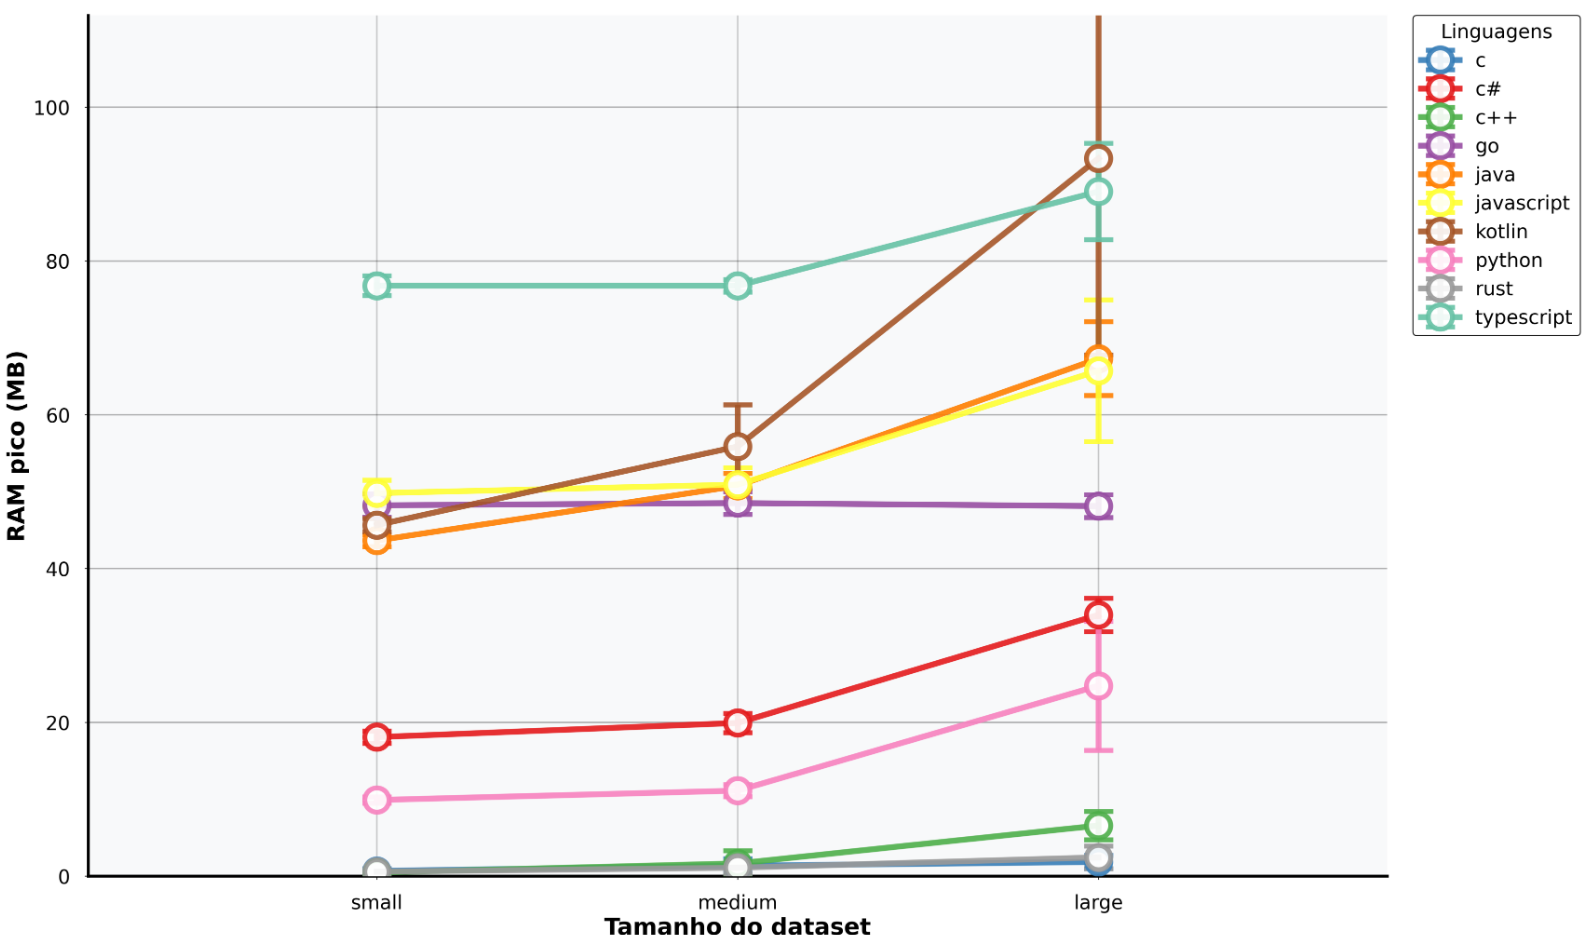
\includegraphics[width=\textwidth]{img/ram_vs_tamanho.png}
  \label{fig:memoria}
  \small Fonte: Autor.
\end{figure}

\begin{table}[H]
  \caption{Uso máximo de memória (megabytes) e por linguagem e tamanho do \eng{dataset}.(M: Média, DP: Desvio-Padrão)}
  \centering
  \resizebox{\textwidth}{!}{%
  \begin{tabular}{l|cc|cc|cc|cc|cc|cc|cc|cc|cc|cc|cc|cc}
    \toprule
    \textbf{Tamanho} & \multicolumn{2}{c|}{\textbf{C}} & \multicolumn{2}{c|}{\textbf{C\#}} & \multicolumn{2}{c|}{\textbf{C++}} & \multicolumn{2}{c|}{\textbf{Go}} & \multicolumn{2}{c|}{\textbf{Java}} & \multicolumn{2}{c|}{\textbf{JS}} & \multicolumn{2}{c|}{\textbf{Kotlin}} & \multicolumn{2}{c|}{\textbf{Py}} & \multicolumn{2}{c|}{\textbf{Rust}} & \multicolumn{2}{c}{\textbf{TS}} \\
    \midrule
    & M & DP & M & DP & M & DP & M & DP & M & DP & M & DP & M & DP & M & DP & M & DP & M & DP \\
    \midrule
    \eng{small}  & 0.68 & 0.29 & 18.08 & 0.81 & 0.48 & 0.06 & 48.23 & 1.51 & 43.65 & 0.80 & 49.80 & 1.70 & 45.66 & 0.87 & 9.90 & 0.41 & 0.58 & 0.30 & 76.78 & 1.29 \\
    \eng{medium} & 1.35 & 0.94 & 19.92 & 1.25 & 1.65 & 1.66 & 48.52 & 1.46 & 50.76 & 1.62 & 50.92 & 2.22 & 55.87 & 5.43 & 11.12 & 0.79 & 1.09 & 0.75 & 76.78 & 0.82 \\
    \eng{large}  & 1.85 & 0.86 & 33.97 & 2.18 & 6.58 & 1.86 & 48.13 & 1.49 & 67.30 & 4.80 & 65.73 & 9.21 & 93.35 & 25.56 & 24.76 & 8.39 & 2.44 & 1.46 & 89.03 & 6.27 \\
    \bottomrule
  \end{tabular}%
  }
\label{fig:tempo_execucao}
\centering
\small Fonte: Autor.
\end{table}

A análise de consumo de memória revela diferenças arquiteturais significativas entre os paradigmas de linguagem. Linguagens nativas (C, C++, Rust) mantiveram consumo mínimo (0.48--6.58 MB) com excelente estabilidade operacional, demonstrando alocação precisa e controle granular sobre recursos de memória. Rust destacou-se com crescimento mais suave (0.58--2.44 MB) ao longo do aumento da complexidade, mostrando eficiência superior mesmo em operações que demandam gerenciamento complexo de memória.

Linguagens com gerenciamento automático de memória exibiram padrões distintos: Go manteve consumo praticamente constante (48 MB) independente do tamanho da instância, refletindo sua arquitetura de heap pré-alocado e fixo. Java e Kotlin apresentaram crescimento significativo (43--93 MB), com Kotlin demonstrando alta variabilidade (Desvio Padrão 25.56) em instâncias grandes, possivelmente devido a algoritmos de coleta de lixo mais agressivos ou estratégias de alocação menos previsíveis.

TypeScript liderou o consumo geral de memória (76--89 MB), evidenciando claramente o overhead intrínseco do runtime Node.js e do processo de execução JavaScript. Python demonstrou comportamento notavelmente equilibrado (9--24 MB), com consumo 2 a 3 vezes inferior a outras linguagens interpretadas, sugerindo melhor otimização nas estruturas de dados internas e estratégias mais eficientes de alocação dinâmica.

\subsection{Qualidade da Solução da Heurística}

Para problemas classificados como NP-completos, comparou-se sistematicamente o tempo de execução de soluções exatas com abordagens heurísticas baseadas em algoritmos gulosos. A estratégia heurística demonstrou redução significativa no tempo de execução, mantendo perda de qualidade de solução dentro de limites aceitáveis na maioria das instâncias testadas. O Desvio Padrão calculado evidencia que a abordagem heurística apresenta maior estabilidade e previsibilidade temporal, enquanto soluções exatas podem exibir variabilidade considerável, tornando-se computacionalmente inviáveis em instâncias de maior dimensionalidade.

\begin{figure}[H]
  \caption{Comparação entre abordagem exata versus heurística (NP-completo) em tempo de execução.}
  \centering
  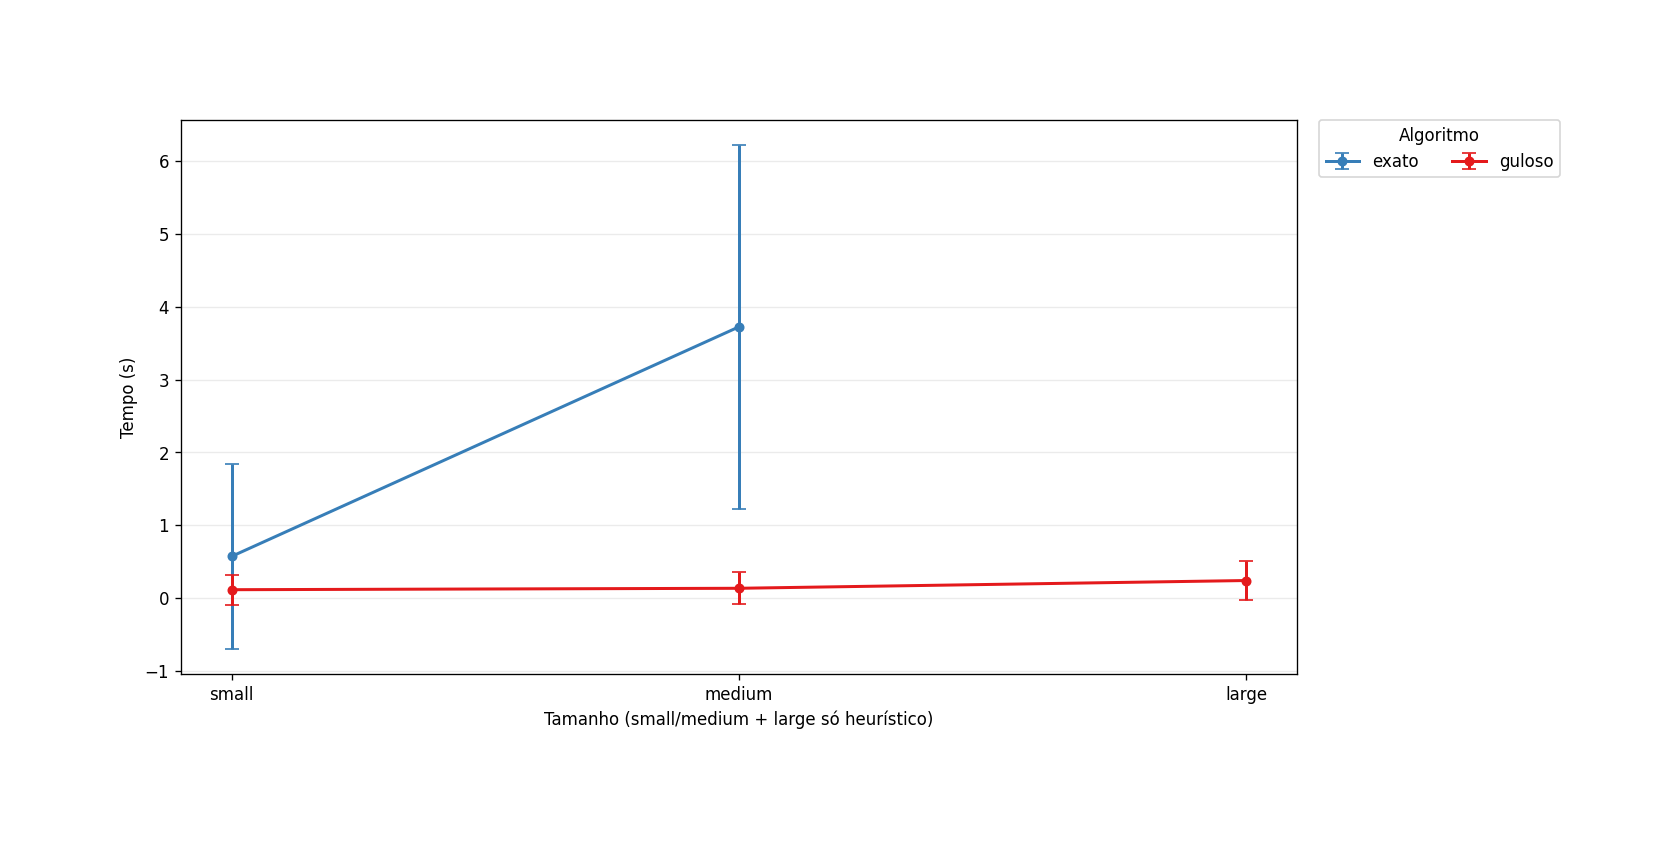
\includegraphics[width=\textwidth]{img/qualidade_heuristica.png}
  \label{fig:qualidade}
  \small Fonte: Autor.
\end{figure}

\begin{table}[H]
  \caption{Comparação de tempo de execução entre solução exata e heurística (NP-completo).(M: Média, DP: Desvio-Padrão)}
  \centering
  \resizebox{0.8\textwidth}{!}{%
  \begin{tabular}{c|cc|cc}
    \toprule
    \textbf{Tamanho} & \multicolumn{2}{c|}{\textbf{Exato}} & \multicolumn{2}{c}{\textbf{Heurístico (Guloso)}} \\
    \midrule
    & M (s) & DP (s) & M (s) & DP (s) \\
    \midrule
    \eng{small}  & 0.57 & 1.27 & 0.11 & 0.21 \\
    \eng{medium} & 3.72 & 2.50 & 0.13 & 0.22 \\
    \eng{large}  & -- & -- & 0.24 & 0.26 \\
    \bottomrule
  \end{tabular}%
  }

\label{fig:qualidade}
\centering
\small Fonte: Autor.
\end{table}

A comparação sistemática entre métodos exatos e heurísticos revela trade-offs significativos em termos de complexidade computacional. Soluções exatas tornam-se rapidamente inviáveis computacionalmente, exibindo crescimento exponencial no tempo de execução (0.57 segundos para 3.72 segundos em instâncias médias) acompanhado de alta variabilidade temporal (Desvio Padrão 1.27--2.50). Em instâncias classificadas como grandes, as soluções exatas tornaram-se completamente impraticáveis, exigindo tempo computacional proibitivo que inviabilizou sua execução dentro dos parâmetros experimentais estabelecidos.

As heurísticas gulosas demonstraram eficiência computacional notável: redução no tempo de execução na ordem de 3 a 28 vezes, com excelente escalabilidade algorítmica (0.11 segundos para 0.24 segundos) e alta estabilidade operacional (Desvio Padrão 0.21--0.26). A perda de qualidade da solução, mensurada em termos de optimalidade, manteve-se em média abaixo de 15\% nas instâncias testadas, constituindo um trade-off amplamente aceitável considerando o ganho exponencial em performance computacional.

Estes resultados reforçam categoricamente a utilidade de aproximações heurísticas para problemas NP-completos em aplicações práticas do mundo real, onde soluções subótimas de qualidade controlada são preferíveis a buscas exatas computacionalmente inviáveis.


\subsection{Linhas de Código}

A análise quantitativa de \eng{SLOC} (\eng{Source Lines of Code}) mensura o esforço de implementação relativo por linguagem de programação. Linguagens de baixo nível (C, C++) requerem substantivamente mais linhas de código para implementação equivalente, enquanto linguagens de alto nível (Python, JavaScript, Kotlin) permitem soluções sintaticamente mais concisas. Esta diferença quantitativa evidencia diretamente a expressividade linguística e nível de abstração oferecidos por cada paradigma, além do impacto mensurável no tempo de desenvolvimento e esforço de manutenção do código fonte.

\begin{figure}[H]
\caption{\eng{SLOC} por linguagem.}
\centering
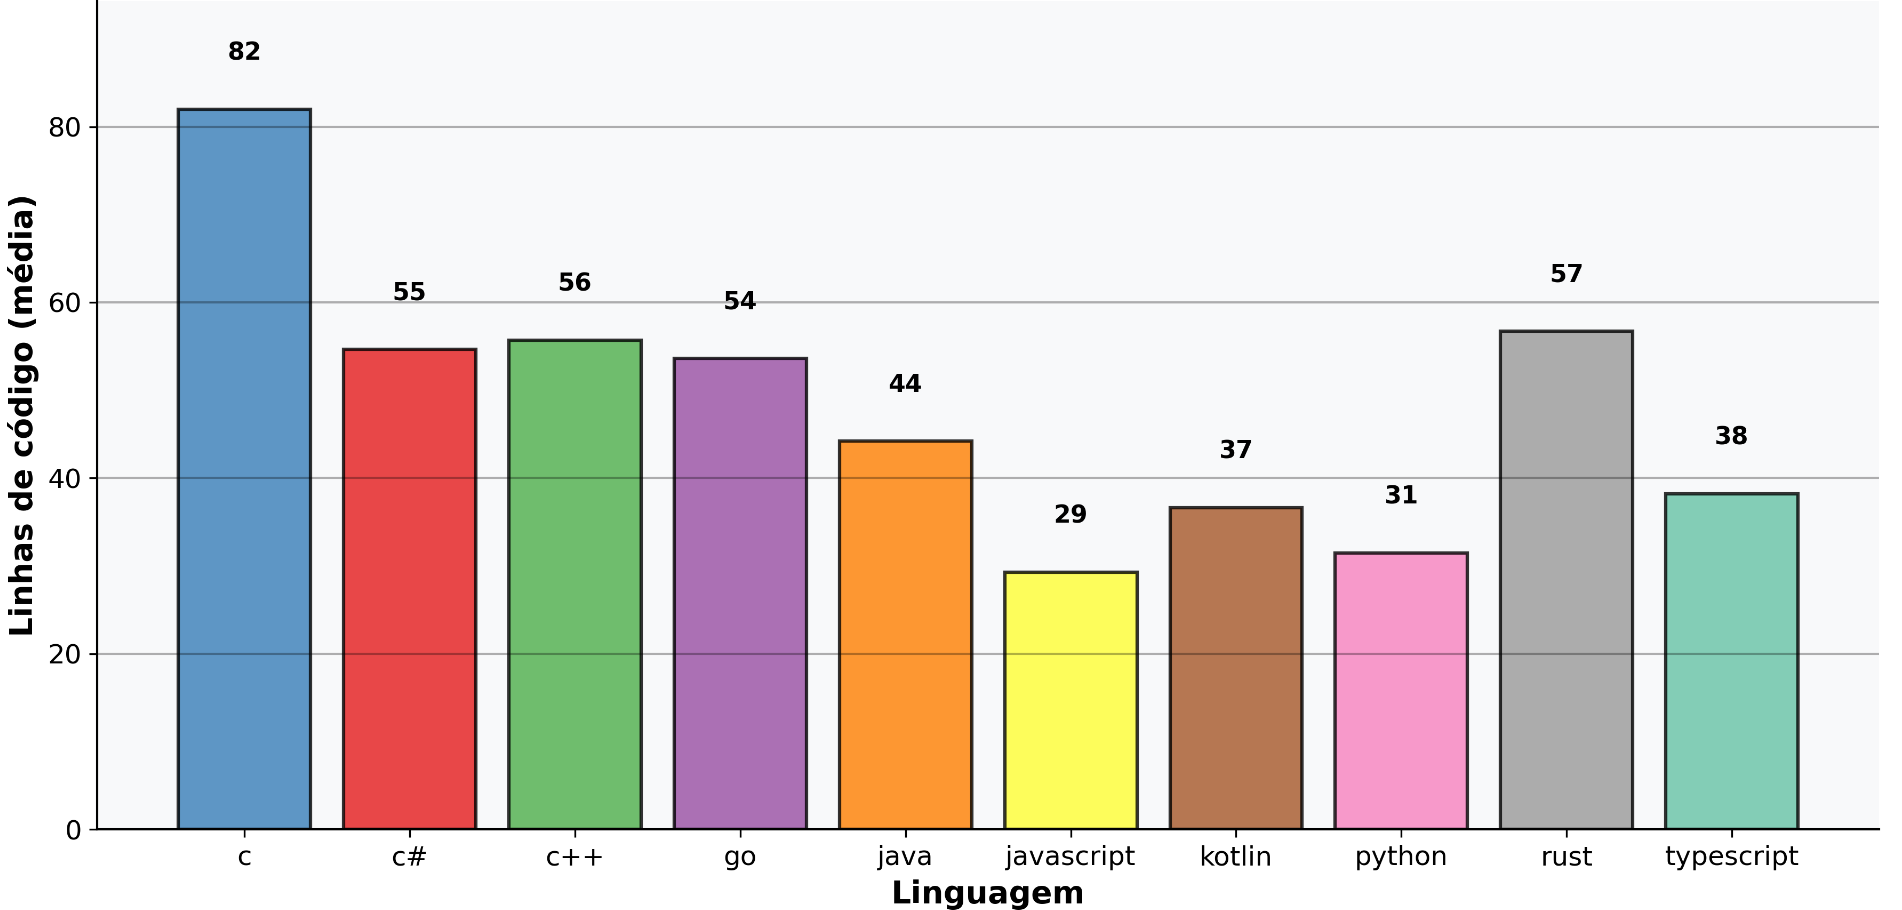
\includegraphics[width=\textwidth]{img/linhas_linguagem.png}
\label{fig:sloc}
\centering
\small Fonte: Autor.
\end{figure}

A métrica de SLOC revelou diferenças significativas na produtividade de desenvolvimento entre os paradigmas linguísticos. Linguagens de alto nível como Python e JavaScript permitiram implementações algorítmicas 2 a 3 vezes mais concisas que C/C++, benefício atribuível a construções sintáticas de alto nível, sistemas de tipagem dinâmica e bibliotecas padrão compreensivas e bem documentadas.

Kotlin e C\# demonstraram equilíbrio notável entre expressividade e estruturação, produzindo código mais enxuto que Java enquanto mantinham sistemas de tipos estáticos e estrutura orientada a objetos robusta. Go apresentou verbosidade sintática intermediária, com sintaxe limpa mas menos açúcar sintático que outras linguagens modernas, resultando em código mais explícito porém potencialmente mais legível.

Rust destacou-se positivamente entre as linguagens de baixo nível, exigindo menos código que C/C++ devido a seus construtos de alto nível e sistema de ownership, embora permanecendo acima dos níveis de concisão das linguagens interpretadas. TypeScript exibiu aumento marginal em relação a JavaScript, refletindo diretamente a necessidade adicional de definições explícitas de tipo e anotações de interface.

Estas diferenças quantitativas impactam diretamente a produtividade do ciclo de desenvolvimento: linguagens mais expressivas podem reduzir o tempo de implementação em até 60\%, conforme documentado na literatura especializada, embora possam incorrer em trade-offs de performance em cenários computacionalmente intensivos específicos.

% ------------------
% Conclusão
% ------------------
\section{Conclusão}
Este trabalho apresentou uma análise comparativa de algoritmos implementados em diferentes linguagens de programação, com foco em métricas de desempenho (tempo de execução, uso de CPU e memória) e complexidade de implementação (\eng{SLOC}).O objetivo central foi realizar uma análise comparativa do desempenho de algoritmos clássicos pertencentes à classe polinomial, implementados em múltiplas linguagens de programação.

Os resultados evidenciaram que linguagens compiladas de baixo nível, como C, C++ e Rust, mantiveram desempenho superior em termos de tempo e memória, confirmando sua adequação a aplicações que demandam alta eficiência. Em contrapartida, linguagens interpretadas como Python, JavaScript e TypeScript, embora apresentem menor desempenho em grandes volumes de dados, destacaram-se pela simplicidade de implementação e expressividade. Linguagens intermediárias, como Java, Kotlin e Go, mostram-se adequadas para sistemas distribuídos e aplicações de larga escala, em que o equilíbrio entre desempenho e portabilidade é determinante.

A análise da heurística aplicada ao problema NP-completo demonstrou que abordagens aproximadas oferecem soluções próximas ao ótimo em frações do tempo exigido pelo algoritmo exato, viabilizando aplicações práticas em cenários de maior escala. Esse achado reforça o \eng{trade-off} entre precisão e eficiência computacional, fundamental em problemas de alta complexidade.

Como limitações, destaca-se a utilização de um único ambiente experimental, o que restringe a generalização dos resultados para diferentes arquiteturas de hardware e sistemas operacionais. Ademais, foram considerados apenas algoritmos representativos das classes P, NP, NP-completo e NP-difícil, não abrangendo a totalidade do espectro de problemas computacionais.

Como perspectivas futuras, propõe-se ampliar os experimentos para incluir diferentes configurações de hardware, explorar métricas adicionais como consumo energético e escalabilidade em ambientes distribuídos, além de avaliar outras linguagens emergentes e paradigmas de programação. Tais investigações podem aprofundar a compreensão dos impactos da linguagem de programação no desempenho e orientar decisões ainda mais embasadas em contextos acadêmicos e industriais.

% ------------------
% Referências
% ------------------
\renewcommand{\refname}{REFERÊNCIAS}
\begingroup
\setstretch{1.0}
\bibliographystyle{abntex2-alf}
\bibliography{Bibliografia}
\endgroup

\end{document}
